\documentclass{article}
\usepackage[UTF8]{ctex}
\usepackage[tc]{titlepic}
\usepackage{titlesec}
\usepackage{cite}
\usepackage{fancyhdr}
\usepackage{booktabs}
\usepackage{graphicx}
\usepackage{geometry}
\usepackage[section]{placeins}
\geometry{a4paper,scale=0.8}
\pagestyle{fancy}

\lhead{第 x 次作业\\\today}
\chead{中国科学技术大学\\数学建模课程}

\rhead{Assignment x\\ {\CTEXoptions[today=old]\today}}
\newcommand{\upcite}[1]{\textsuperscript{\cite{#1}}}

\titleformat*{\section}{\bfseries\Large}
\titleformat*{\subsection}{\bfseries\large}

\title{\bfseries 作业名字xxx}
\author{张三 \quad  课程ID \quad  学号}

\begin{document}
\maketitle
\begin{abstract}
    你的文章摘要
\end{abstract}
\clearpage
% \setcounter{secnumdepth}{1}
 \setcounter{section}{1}
\section*{\centerline{一、前言(问题的提出)}}
\subsection{子标题1}
    你的问题描述xxxx  \\
\subsection{子标题2}
    xxxxxxx  
 \setcounter{section}{2}
\section*{\centerline{二、相关工作}}
    引用文献\upcite{946629}
 \setcounter{section}{3}
\section*{\centerline{三、问题分析}}
    你的问题分析
    \subsection{分析1}
    \subsection{分析2}
 \setcounter{section}{4}
\section*{\centerline{四、建模的假设}}
    你的模型假设 
    \subsection{假设1}
    \subsection{假设2}

 \setcounter{section}{5}
 \section*{\centerline{五、符号说明}}
 \begin{table}[t]
    \caption{\textbf{符号说明}}%标题
    \centering%把表居中
    \begin{tabular}{ccc}%内容全部居中
    \toprule%第一道横线
    符号&说明&单位 \\
    \midrule%第二道横线 
    $\alpha$ &description of $alpha$ & xx \\
    $\beta$ & description of $beta$ & xx \\
    \bottomrule%第三道横线
    \end{tabular}
\end{table}

 \setcounter{section}{6}
\section*{\centerline{六、数学模型建立}}
    你建立的数学模型和算法的描述 

 \setcounter{section}{7}
\section*{\centerline{七、结果(与对比)}}
    你的算法产生的结果,如果有多种算法产生的结果,需要做对比。
    \subsection{结果展示}
    引用图片
    \begin{figure}[h]
        \centering %居中
        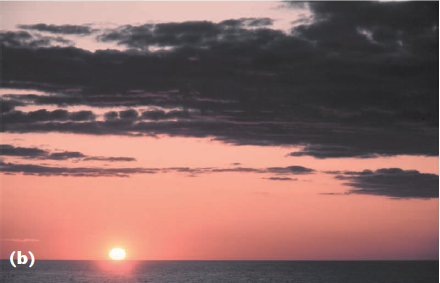
\includegraphics[scale=0.5]{eg.png}
        \caption{figure example}
    \end{figure}
    \subsection{结果对比}

 \setcounter{section}{8}
\section*{\centerline{八、结论}}
    实验产生了何种结论  

 \setcounter{section}{9}
\section*{\centerline{九、问题}}
    解决问题的过程中你是否发现的新的问题,或者算法仍然存在改进的地方?  

\bibliographystyle{ieeetr}
\bibliography{refer}

\end{document}